\documentclass[a4paper, 11pt]{article}
\usepackage{amsmath}
\usepackage{graphicx}
\usepackage{geometry}
\usepackage{listings}
\geometry{scale=0.8}
\linespread{1.5}
\usepackage{hyperref}
\usepackage{longtable}

\title{
\normalfont \normalsize
\textsc{School of Data and Computer Science, Sun Yat-sen University} \\ [25pt] %textsc small capital letters
\rule{\textwidth}{0.5pt} \\[0.4cm] % Thin top horizontal rule
\huge  P01 Pacman Game \\ % The assignment title
\rule{\textwidth}{2pt} \\[0.5cm] % Thick bottom horizontal rule
\author{16000001 San Zhang, 16000002 Si Li}
\date{\normalsize\today}
}

\begin{document}
\maketitle
\tableofcontents
\newpage
\section{Search in Pacman}
\subsection{Introduction}
In this section, your Pacman agent will find paths through his maze world, both to reach a particular location and to collect food efficiently. You will build general search algorithms and apply them to Pacman scenarios.

\rule{\textwidth}{0.5pt}

\textbf{Files you'll edit:}

\begin{tabular}{ll}
  \textsf{search.py} &  Where all of your search algorithms will reside.\\
  \textsf{searchAgents.py} & Where all of your search-based agents will reside.
\end{tabular}

\rule{\textwidth}{0.5pt}

\textbf{Files you might want to look at:}

\begin{tabular}{ll}
  \textsf{pacman.py} & The main file that runs Pacman games. This file describes a Pacman GameState type.\\
  \textsf{game.py} &	The logic behind how the Pacman world works.\\
  & This file describes several supporting types like AgentState, Agent, Direction, and Grid.\\
  \textsf{util.py} &	Useful data structures for implementing search algorithms.
\end{tabular}

\rule{\textwidth}{0.5pt}

\textbf{Supporting files you can ignore:}

\begin{tabular}{ll}
  \textsf{graphicsDisplay.py} &	Graphics for Pacman\\
  \textsf{graphicsUtils.py} &	Support for Pacman graphics\\
  \textsf{textDisplay.py} &	ASCII graphics for Pacman\\
  \textsf{ghostAgents.py} &	Agents to control ghosts\\
  \textsf{keyboardAgents.py} &	Keyboard interfaces to control Pacman\\
  \textsf{layout.py} &	Code for reading layout files and storing their contents\\
  \textsf{autograder.py} &	Project autograder\\
  \textsf{testParser.py} &	Parses autograder test and solution files\\
  \textsf{testClasses.py} &	General autograding test classes\\
  \textsf{test\_cases/} &	Directory containing the test cases for each question\\
  \textsf{searchTestClasses.py} &	Specific autograding test classes\\
\end{tabular}

\rule{\textwidth}{0.5pt}

\textbf{Files to Edit and Submit:} You will fill in portions of \textsf{search.py} and \textsf{searchAgents.py} during the assignment. You should submit these files with your code and comments. Please do not change the other files in this distribution or submit any of our original files other than these files.

\textbf{Evaluation:} Your code will be autograded for technical correctness. Please do not change the names of any provided functions or classes within the code, or you will wreak havoc on the autograder.
\subsection{Welcome to Pacman}
After downloading the code (search.zip), unzipping it, and changing to the directory, you should be able to play a game of Pacman by typing the following at the command line:

\texttt{python pacman.py}

The simplest agent in \textsf{searchAgents.py} is called the \textsf{GoWestAgent}, which always goes West (a trivial reflex agent). This agent can occasionally win:

\texttt{python pacman.py --layout testMaze --pacman GoWestAgent}

But, things get ugly for this agent when turning is required:

\texttt{python pacman.py --layout tinyMaze --pacman GoWestAgent}

If Pacman gets stuck, you can exit the game by typing \texttt{CTRL-c} into your terminal.

Soon, your agent will solve not only \textsf{tinyMaze}, but any maze you want.

Note that \textsf{pacman.py} supports a number of options that can each be expressed in a long way (e.g., \texttt{--layout}) or a short way (e.g., \texttt{-l}). You can see the list of all options and their default values via:

\texttt{python pacman.py -h}

Also, all of the commands that appear in this project also appear in \textsf{commands.txt}, for easy copying and pasting.
\subsection{Question 1: A* search ( 3 points)}
Implement A* graph search in the empty function \textsf{aStarSearch} in \textsf{search.py}. A* takes a heuristic function as an argument. Heuristics take two arguments: a state in the search problem (the main argument), and the problem itself (for reference information). The \textsf{nullHeuristic} heuristic function in \textsf{search.py} is a trivial example.

You can test your A* implementation on the original problem of finding a path through a maze to a fixed position using the Manhattan distance heuristic (implemented already as \textsf{manhattanHeuristic} in \textsf{searchAgents.py}).

\texttt{python pacman.py -l bigMaze -z .5 -p SearchAgent -a fn=astar,heuristic=manhattanHeuristic}

\subsection{Question 2: Corners Problem: Heuristic ( 3 points)}
\textit{Note: Make sure to complete Question 1 before working on Question 2, because Question 2 builds upon your answer for Question 1.}

Implement a non-trivial, consistent heuristic for the \textsf{CornersProblem} in \textsf{cornersHeuristic}.

\texttt{python pacman.py -l mediumCorners -p AStarCornersAgent -z 0.5}

\textit{Note:} \textsf{AStarCornersAgent} is a shortcut for

\texttt{-p SearchAgent -a fn=aStarSearch,prob=CornersProblem,heuristic=cornersHeuristic.}

\textbf{\textit{Admissibility vs. Consistency:}} Remember, heuristics are just functions that take search states and return numbers that estimate the cost to a nearest goal. More effective heuristics will return values closer to the actual goal costs. To be admissible, the heuristic values must be lower bounds on the actual shortest path cost to the nearest goal (and non-negative). To be consistent, it must additionally hold that if an action has cost c, then taking that action can only cause a drop in heuristic of at most c.

Remember that admissibility isn't enough to guarantee correctness in graph search -- you need the stronger condition of consistency. However, admissible heuristics are usually also consistent, especially if they are derived from problem relaxations. Therefore it is usually easiest to start out by brainstorming admissible heuristics. Once you have an admissible heuristic that works well, you can check whether it is indeed consistent, too. The only way to guarantee consistency is with a proof. However, inconsistency can often be detected by verifying that for each node you expand, its successor nodes are equal or higher in in f-value. Moreover, if UCS and A* ever return paths of different lengths, your heuristic is inconsistent. This stuff is tricky!

\textbf{\textit{Non-Trivial Heuristics:}} The trivial heuristics are the ones that return zero everywhere (UCS) and the heuristic which computes the true completion cost. The former won't save you any time, while the latter will timeout the autograder. You want a heuristic which reduces total compute time, though for this assignment the autograder will only check node counts (aside from enforcing a reasonable time limit).

\textbf{\textit{Grading:}} Your heuristic must be a non-trivial non-negative consistent heuristic to receive any points. Make sure that your heuristic returns 0 at every goal state and never returns a negative value. Depending on how few nodes your heuristic expands, you'll be graded:

\begin{center}
\begin{tabular}{||l||l||}
  \hline\hline
  Number of nodes expanded & Grade\\
  \hline\hline
  more than 2000 & 0/3\\
  \hline\hline
  at most 2000 & 1/3\\
  \hline\hline
  at most 1600 & 2/3\\
  \hline\hline
  at most 1200 & 3/3\\
  \hline\hline
\end{tabular}
\end{center}
\textit{Remember:} If your heuristic is inconsistent, you will receive no credit, so be careful!
\subsection{Question 3: Eating All The Dots ( 4 points)}
Now we'll solve a hard search problem: eating all the Pacman food in as few steps as possible. For this, we'll need a new search problem definition which formalizes the food-clearing problem: \textsf{FoodSearchProblem} in \textsf{searchAgents.py} (implemented for you). A solution is defined to be a path that collects all of the food in the Pacman world. For the present project, solutions do not take into account any ghosts or power pellets; solutions only depend on the placement of walls, regular food and Pacman. (Of course ghosts can ruin the execution of a solution! We'll get to that in the next project.) If you have written your general search methods correctly, A* with a null heuristic (equivalent to uniform-cost search) should quickly find an optimal solution to testSearch with no code change on your part (total cost of 7).

\texttt{python pacman.py -l testSearch -p AStarFoodSearchAgent}
Note: AStarFoodSearchAgent is a shortcut for \texttt{-p SearchAgent -a fn=astar,prob=FoodSearchProblem,heuristic=foodHeuristic}.

\textit{Note:} Make sure to complete Question 1 before working on Question 3, because Question 3 builds upon your answer for Question 1.

Fill in \textsf{foodHeuristic} in \textsf{searchAgents.py} with a consistent heuristic for the \textsf{FoodSearchProblem}. Try your agent on the \textsf{trickySearch board}:

\texttt{python pacman.py -l trickySearch -p AStarFoodSearchAgent}

Any non-trivial non-negative consistent heuristic will receive 1/4. Make sure that your heuristic returns 0 at every goal state and never returns a negative value. Depending on how few nodes your heuristic expands, you'll get additional points:

\begin{center}
\begin{tabular}{||l||l||}
  \hline\hline
  Number of nodes expanded & Grade\\
  \hline\hline
  more than 15000 & 1/4\\
  \hline\hline
  at most 15000 & 2/4\\
  \hline\hline
  at most 12000 & 3/4\\
  \hline\hline
  at most 9000 & 4/4 (full credit; medium)\\
  \hline\hline
  at most 7000 & 5/4 (optional extra credit; hard)\\
  \hline\hline
\end{tabular}
\end{center}
%---------------------------------------------------------------------------------------------
\newpage
\section{Multi-Agent Pacman}
\subsection{Introduction}
In this section, you will design agents for the classic version of Pacman, including ghosts. Along the way, you will implement both minimax and $\alpha-\beta$ pruning. The code for this section contains the folowing files, available in \textsf{multiagent.zip}.

\rule{\textwidth}{0.5pt}

\textbf{Files you'll edit:}

\begin{tabular}{ll}
  \textsf{multiAgents.py} &	Where all of your multi-agent search agents will reside.\\
  \textsf{pacman.py} &	The main file that runs Pacman games.\\
  & This file also describes a Pacman GameState type,\\
                          & which you will use extensively in this project\\
  \textsf{game.py}	& The logic behind how the Pacman world works. \\
                          & This file describes several supporting types like\\
                          & AgentState, Agent, Direction, and Grid.\\
  \textsf{util.py} &	Useful data structures for implementing search algorithms.
\end{tabular}

\rule{\textwidth}{0.5pt}

\textbf{Files you can ignore:}

\begin{tabular}{ll}
  \textsf{graphicsDisplay.py} &	Graphics for Pacman\\
  \textsf{graphicsUtils.py}&	Support for Pacman graphics\\
  \textsf{textDisplay.py}&	ASCII graphics for Pacman\\
  \textsf{ghostAgents.py}&	Agents to control ghosts\\
  \textsf{keyboardAgents.py}&	Keyboard interfaces to control Pacman\\
  \textsf{layout.py}&	Code for reading layout files and storing their contents\\
  \textsf{autograder.py}&	Project autograder\\
  \textsf{testParser.py}&	Parses autograder test and solution files\\
  \textsf{testClasses.py}&	General autograding test classes\\
  \textsf{test\_cases/}&	Directory containing the test cases for each question\\
  \textsf{multiagentTestClasses.py}&	Specific autograding test classes
\end{tabular}

\rule{\textwidth}{0.5pt}

\textbf{Files to Edit and Submit:} You will fill in portions of \textsf{multiAgents.py} during the assignment. You should submit this file with your code and comments. Please do not change the other files in this distribution or submit any of our original files other than this file.

\textbf{Evaluation:} Your code will be autograded for technical correctness. Please do not change the names of any provided functions or classes within the code, or you will wreak havoc on the autograder.
\subsection{Multi-Agent Pacman}
First, play a game of classic Pacman:

\texttt{python pacman.py}

Now, run the provided \textsf{ReflexAgent} in \textsf{multiAgents.py}:

\texttt{python pacman.py -p ReflexAgent}

Note that it plays quite poorly even on simple layouts:

\texttt{python pacman.py -p ReflexAgent -l testClassic}

Inspect its code (in \textsf{multiAgents.py}) and make sure you understand what it's doing.
\subsection{Question 4: Minimax ( 5 points)}
Now you will write an adversarial search agent in the provided\textsf{ MinimaxAgent} class stub in \textsf{multiAgents.py}. Your minimax agent should work with any number of ghosts, so you'll have to write an algorithm that is slightly more general than what you've previously seen in lecture. In particular, your minimax tree will have multiple min layers (one for each ghost) for every max layer.

Your code should also expand the game tree to an arbitrary depth. Score the leaves of your minimax tree with the supplied \textsf{self.evaluationFunction}, which defaults to \textsf{scoreEvaluationFunction}. \textsf{MinimaxAgent} extends \textsf{MultiAgentSearchAgent}, which gives access to \textsf{self.depth} and \textsf{self.evaluationFunction}. Make sure your minimax code makes reference to these two variables where appropriate as these variables are populated in response to command line options.

\textit{Important:} A single search ply is considered to be one Pacman move and all the ghosts' responses, so depth 2 search will involve Pacman and each ghost moving two times.

\textit{Grading:} We will be checking your code to determine whether it explores the correct number of game states. This is the only way reliable way to detect some very subtle bugs in implementations of minimax. As a result, the autograder will be very picky about how many times you call GameState.generateSuccessor. If you call it any more or less than necessary, the autograder will complain. To test and debug your code, run

\textsf{python autograder.py -q q2}

This will show what your algorithm does on a number of small trees, as well as a pacman game. To run it without graphics, use:

\texttt{python autograder.py -q q2 --no-graphics}

\textbf{\textit{Hints and Observations}}
  \begin{itemize}\setlength{\itemsep}{-\itemsep}
\item The correct implementation of minimax will lead to Pacman losing the game in some tests. This is not a problem: as it is correct behaviour, it will pass the tests.
\item The evaluation function for the pacman test in this part is already written (self.evaluationFunction). You shouldn't change this function, but recognize that now we're evaluating *states* rather than actions, as we were for the reflex agent. Look-ahead agents evaluate future states whereas reflex agents evaluate actions from the current state.
\item The minimax values of the initial state in the minimaxClassic layout are 9, 8, 7, -492 for depths 1, 2, 3 and 4 respectively. Note that your minimax agent will often win (665/1000 games for us) despite the dire prediction of depth 4 minimax.

  \texttt{python pacman.py -p MinimaxAgent -l minimaxClassic -a depth=4}
\item Pacman is always agent 0, and the agents move in order of increasing agent index.
\item All states in minimax should be GameStates, either passed in to getAction or generated via GameState.generateSuccessor. In this project, you will not be abstracting to simplified states.
\item On larger boards such as openClassic and mediumClassic (the default), you'll find Pacman to be good at not dying, but quite bad at winning. He'll often thrash around without making progress. He might even thrash around right next to a dot without eating it because he doesn't know where he'd go after eating that dot. Don't worry if you see this behavior, question 5 will clean up all of these issues.
\item When Pacman believes that his death is unavoidable, he will try to end the game as soon as possible because of the constant penalty for living. Sometimes, this is the wrong thing to do with random ghosts, but minimax agents always assume the worst:

  \texttt{python pacman.py -p MinimaxAgent -l trappedClassic -a depth=3}

\end{itemize}
\subsection{Question 5: $\alpha-\beta$ Pruning ( 5 points)}
Make a new agent that uses $\alpha-\beta$ pruning to more efficiently explore the minimax tree, in \textsf{AlphaBetaAgent}. Again, your algorithm will be slightly more general than the pseudocode from lecture, so part of the challenge is to extend the $\alpha-\beta$ pruning logic appropriately to multiple minimizer agents.

You should see a speed-up (perhaps depth 3 alpha-beta will run as fast as depth 2 minimax). Ideally, depth 3 on \textsf{smallClassic} should run in just a few seconds per move or faster.

\texttt{python pacman.py -p AlphaBetaAgent -a depth=3 -l smallClassic}

The \textsf{AlphaBetaAgent} minimax values should be identical to the \textsf{MinimaxAgent} minimax values, although the actions it selects can vary because of different tie-breaking behavior. Again, the minimax values of the initial state in the \textsf{minimaxClassic} layout are 9, 8, 7 and -492 for depths 1, 2, 3 and 4 respectively.

\textit{Grading:} Because we check your code to determine whether it explores the correct number of states, it is important that you perform alpha-beta pruning without reordering children. In other words, successor states should always be processed in the order returned by \textsf{GameState.getLegalActions}. Again, do not call \textsf{GameState.generateSuccessor} more than necessary.

You must not prune on equality in order to match the set of states explored by our autograder. (Indeed, alternatively, but incompatible with our autograder, would be to also allow for pruning on equality and invoke alpha-beta once on each child of the root node, but this will not match the autograder.)

The pseudo-code below represents the algorithm you should implement for this question.
\begin{figure}[h]
  \centering
  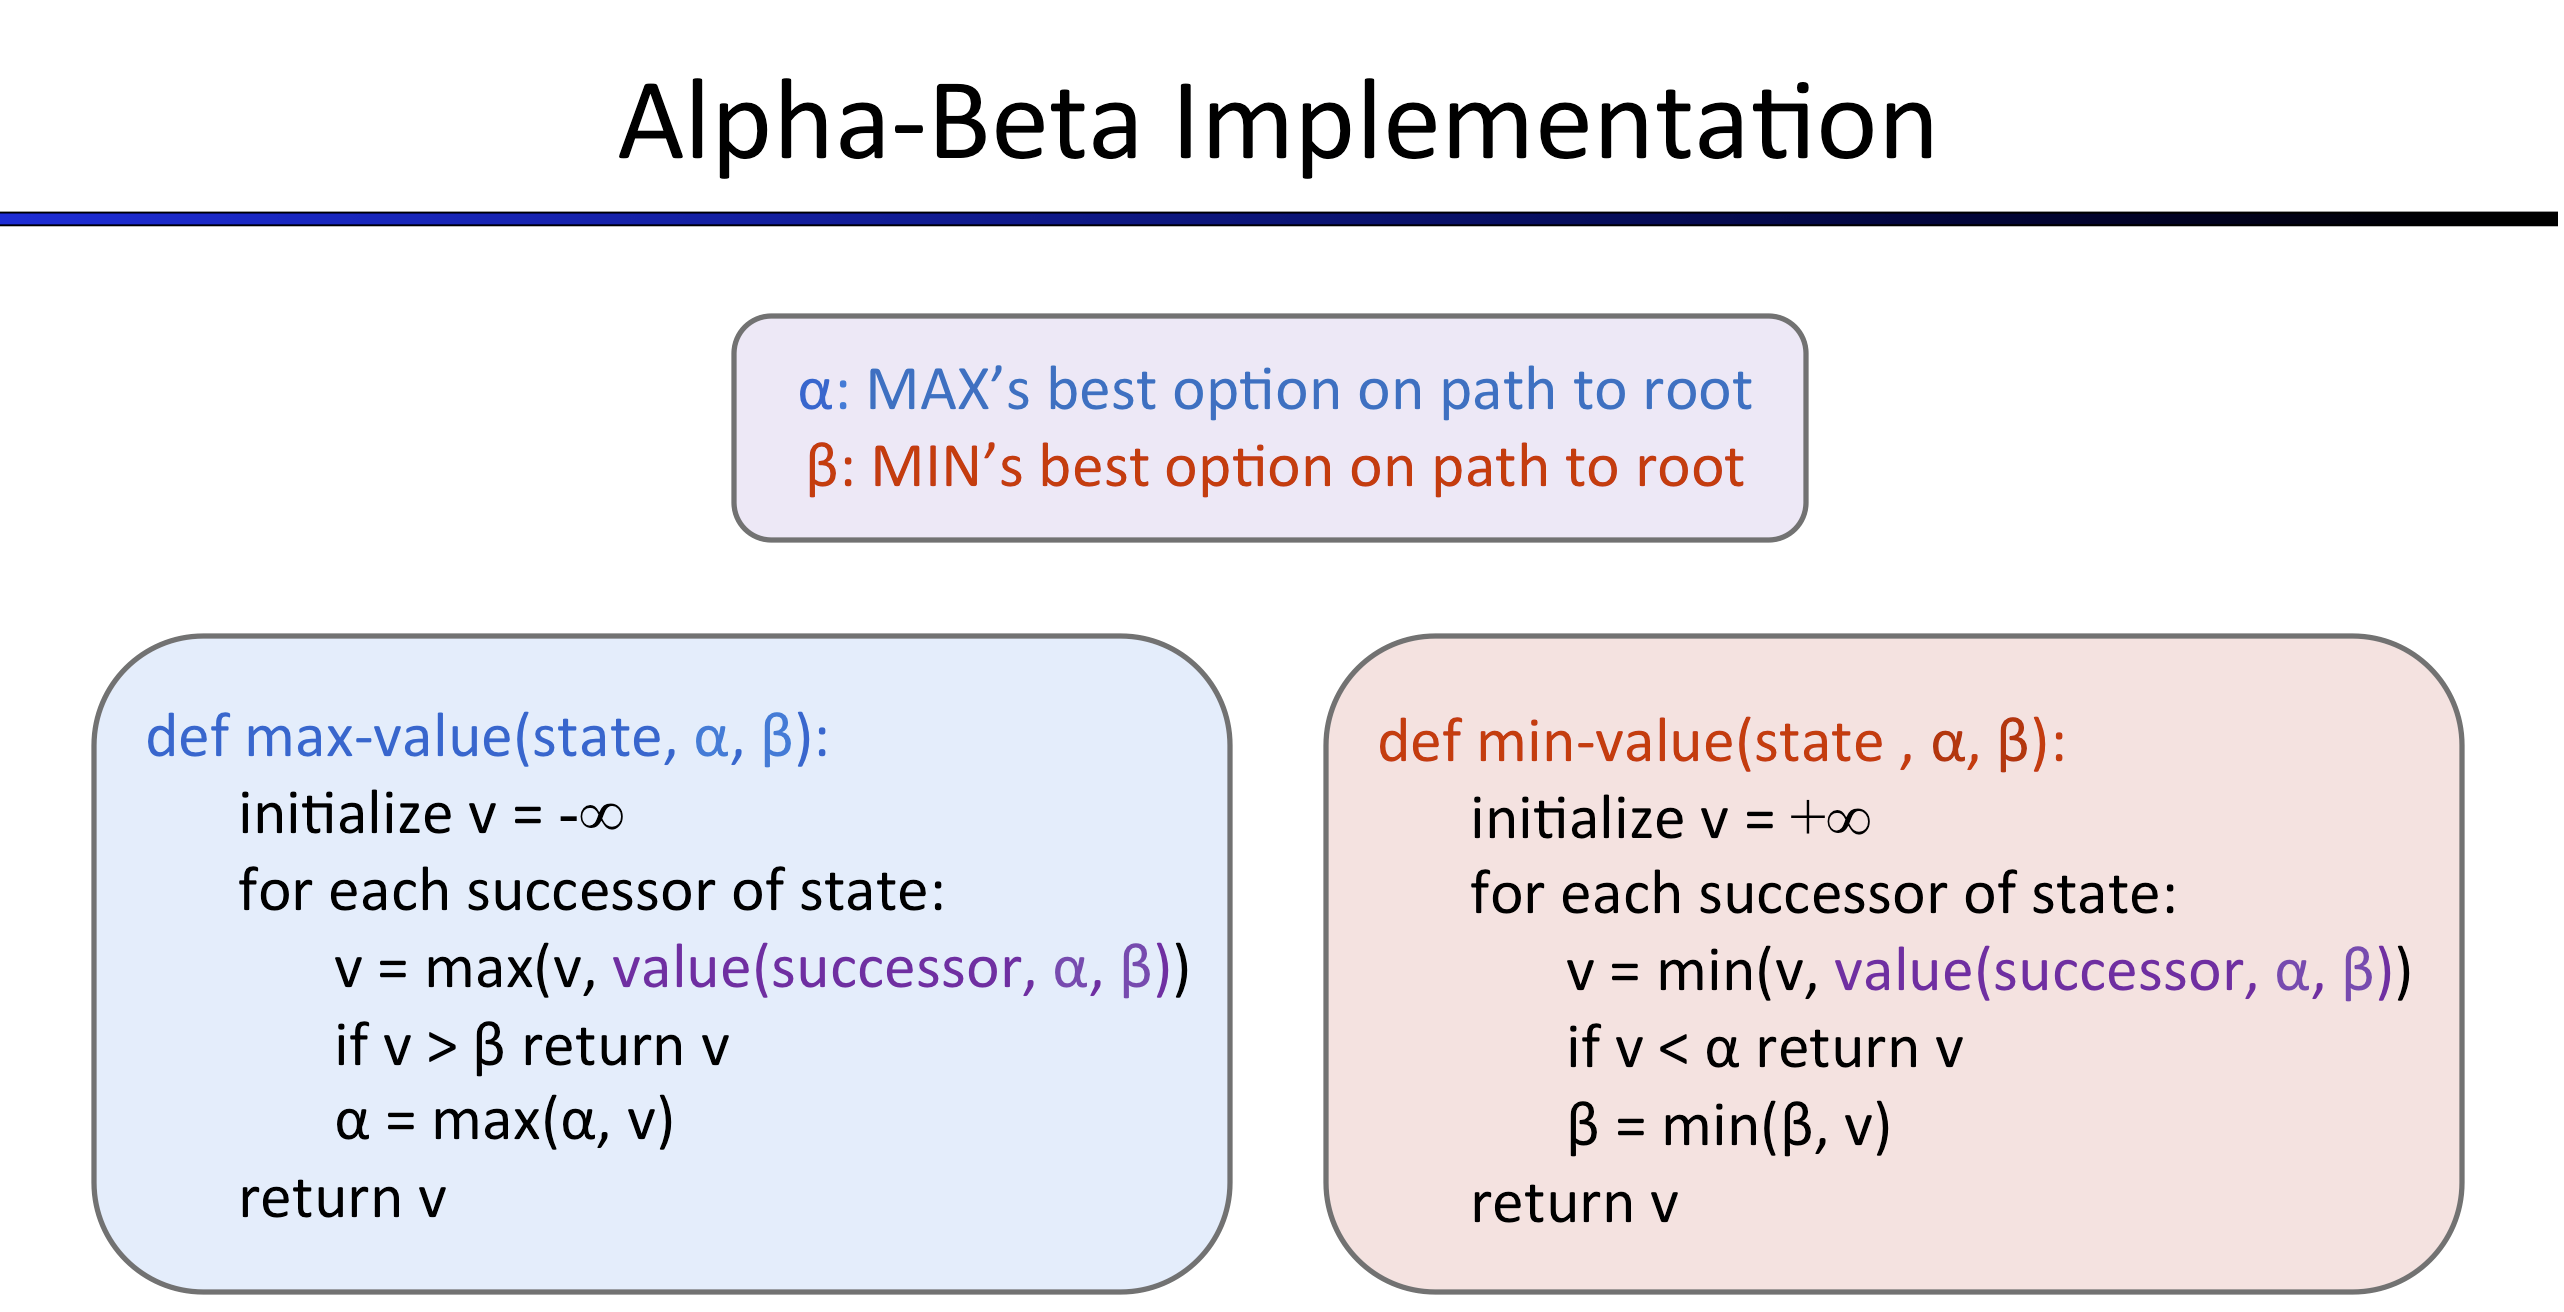
\includegraphics[width=15cm]{alpha-beta-on-inequality}
\end{figure}
\section{Notes}
\begin{enumerate}\setlength{\itemsep}{-\itemsep}
  \item The related files written in Python2 can be found in \textsf{search.zip} and \textsf{multiagent.zip}. You can refer to \url{https://www.liaoxuefeng.com/wiki/001374738125095c955c1e6d8bb493182103fac9270762a000} if you are a noob of Python.
\item You can ask one partner to join you to do together. Please complete the above five questions, and you only need to send \textsf{P01\_YourNumber.zip} which contains the modified \textsf{search.zip} and \textsf{multiagent.zip} to the mailbox(\textsf{ai\_201901@foxmail.com}) before the deadline(2019/10/9 23:59). For this project, you needn't submit the \texttt{pdf} file.
\item Last but not least, you are not alone! If you find yourself stuck on something, contact the TA for help.

\end{enumerate}


\end{document}

